\chapter{Review of Strain Estimation Techniques}\label{review}

Strain is a measure of the deformation of a body, and a building block towards producing quantitative elastic measurements of Young's modulus \cite{wang_optical_2015}. The Young's modulus is defined as the ratio of the axial stress $\sigma$ and strain $\varepsilon$ \cite{kennedy_review_2014}:

\begin{equation}
	E = \frac{\sigma}{\varepsilon}
	\label{youngs_modulus}
\end{equation}

When calculating mechanical properties of tissue, the assumption is made that tissue is linear-elastic, isotropic, and undergoes infinitesimal deformation under loading \cite{kennedy_review_2014}. For small deformations, it is also assumed that the stress due to loading is uniform and axial in depth, such that the local strain may be inversely related to the local Young's modulus.

In compression \ac{oce}, strain is calculated from the measured axial displacement by fitting locally the gradient of the displacement. This relationship between strain and displacement can be thought of as a numerical differentiation process \cite{luo_axial_2004} described by a digital differentiator (a differentiation filter).

To be able to compare between imaging techniques, the resolution of different strain estimation fits must be derived. This resolution can be thought of as the \ac{fwhm} of the impulse response of the strain differentiation filter, which is the output when the input signal is a delta function in the case of a smoothing filter, or a step function for the differentiation filters. This resolution offers a comparative measure of the extent to which the filtering process has blurred objects in the image together. 

\section{Least Squares Approaches}\label{least_squares}
Least squares approach aim to fit a straight line to the phase data by minimising the squared error between the fitted and actual values. The strain value is then taken to be the gradient of this line. The \ac{ols} estimate for the strain value within a fit window of size $m$ is given in \cite{kennedy_strain_2012} as:

\begin{equation}
	\label{ols_strain}
	\varepsilon_i = \sum\limits_{j=i}^{j=i+m-1} \bigg(\frac{\kappa_0 (z_l-z_{l-1})-\kappa_1}{\kappa_0 \kappa_2 - \kappa_1^2} \bigg) u_j
\end{equation}

Where $u_j$ is the displacement at the point, and the simplifying constants $\kappa_x$ are defined as:

\begin{equation}
	\label{ols_k}
	\kappa_x = \sum \limits_{j=i}^{i+m-1} (z_j - z_{i-1})^x \text{   for   } x = 0,1,2
\end{equation}

The estimator is valid only for non-circular (i.e. unwrapped) data, and as such there is a need to unwrap the phase prior to converting it to displacement and performing the least squares estimate.

The \ac{ols} estimate above is a linear operation, however can be extended to weight the contribution of each displacement point based on the quality of its signal. 
The weight in the \ac{wls} estimator is the inverse of the variance of each data point.
The variance of the measured phase difference is equal to the inverse of the \ac{snr} of the \ac{oct} intensity, $SNR_{OCT}$ \cite{goodman_statistical_2015}. Therefore a $\Delta \phi_i$ measurement that has a high $SNR_{OCT}$ has a low variance, and should be assigned more significance in estimating a linear displacement fit. 

\begin{equation}
	\label{wls_w}
	w_i = \frac{1}{\sigma_{u_i}^2} = SNR_{OCT_i}
\end{equation}

Using these weights, the strain estimate using \ac{wls} is given as in \cite{kennedy_strain_2012} by \autoref{wls_strain}:

\begin{equation}
	\label{wls_strain}
	\varepsilon_i = \sum \limits_{j=I}^{i+m-1} \frac{\kappa_0 w_j (z_j - z_{i-1}) u_j - \kappa'_1 w_	j u_j}{\kappa_0 \kappa_2 - (\kappa_1)^2}
\end{equation}

Where in this instance, the $\kappa_x$ constants are given by:

\begin{equation}
	\label{wls_k}
	\kappa_x = \sum \limits_{j=i}^{i+m-1} w_j (z_j - z_{i-1})^x \text{   for   } x=0,1,2
\end{equation}

The \ac{ols} derivative estimator gives the optimal estimate when errors in the data are zero-mean, uncorrelated and have the same variance (by the Gauss-Markove theorem). However, the phase variance in \ac{oct} is related to the highly varying \ac{oct} \ac{snr} and noise in neighbouring pixels. In contrast, \ac{wls} can handle weights (non-uniform variances), which has been shown to improve the strain sensitivity \cite{kennedy_strain_2012}. However this is more computationally expensive, requiring a weight calculation and being a non-linear operation, the consequences of which are discussed in the next section.

\section{\ac{sg} Filtering}\label{sg_filter}
One benefit of the \ac{ols} approach is that it can be implemented as a filter to uniformly sampled data, since it is a linear operation. The \ac{sg} filter \cite{savitzky_smoothing_1964} can be applied to data to smooth it to a linear fit, equivalent to performing a least squares estimate about a window around each point in the data. This filter can be applied to an entire data set by convolving the data and filter together, or multiplying them in the Fourier domain. 
Similarly to how the estimate above for \ac{ols} is derived, the \ac{sg} filter is calculated for the case where the data is sampled at uniform intervals, typically expressed as integer valued points about the centre of the fit window. The \ac{sg} smoothing filter replaces each data point with the \ac{ols} estimate at that point \cite{savitzky_smoothing_1964}. However this can be generalised to a \ac{sg} differentiation filter by instead evaluating the gradient at each point. 
The analytical solution for the first order \ac{sg} differentiation filter is given by \cite{madden_comments_1978}:

\begin{equation}
	\label{sg_coeff}
	C_i = \frac{12 i}{m(m^2-1)}
\end{equation}

Where the $m$ is the integer size of the fit window, and must be odd.

Using this result, not only can this filter be applied much faster by convolution compared to performing sequential looping over all fit windows and using the \ac{ols} summation expression, it can be created very quickly as well. The limitation is that the weight information can no longer be utilised in the convolution process. Also, the \ac{sg} filter can only be applied on the real unwrapped phase difference, since it cannot correct for wrapping events. 

The resolution of the \ac{sg} filter can be derived by analysing it's response to an impulse. Applying the derivative filter of \autoref{sg_coeff} to a unit step response yields the equivalent impulse response of the \ac{sg} filter:

\begin{equation}
	\text{PSF} (C_i)=\frac{6 i^2}{m(m^2-1)}
	\label{impulse_response}
\end{equation}

Which is quadratic in form, and the \ac{fwhm} can be solved for, giving the value in \autoref{sg_fwhm}:

\begin{equation}
	\label{sg_fwhm}
	\text{FWHM}_{SG} = \frac{m}{\sqrt{2}}
\end{equation}

\section{Smoothing Filters}
In most biological signal processing, high frequency noise is a significant degrading factor, one that is amplified in applications such as elastograpy where derivatives are estimated to produce the signal \cite{usui_digital_1982}. As a result, low-pass differentiation filters are ideal signal processing techniques. \ac{ols}, and as a result the \ac{sg} filter acts as a low-pass differentiation filter \cite{luo_axial_2004}, as does \ac{wls}.
Conceptually these filters can be thought of as the combination of an estimate of the derivative of the displacement, followed by smoothing by the impulse response kernel in \ref{impulse_response}. Alternatively, this could be applied as a smoothing of the displacement, followed by an estimate of the derivative. The ordering is signficiant since estimation of the phase difference from the complex variables is not a linear operation (given that it is a complex quotient).

Using this two stage structure, the simplest form of derivative estimation is \ac{fd}, compared to using the \ac{sg} impulse response estimate. However as mentioned in \autoref{least_squares}, the \ac{sg} filter is not optimal for the characteristics of typical \ac{oct} noise.
This raises the question as to whether a different form of smoothing filter may produce better results in estimating strain in \ac{oce}. 

There are a range of smoothing filters to choose from, however this study examines the use of a Gaussian filter, chosen because it has a smooth kernel and a smooth frequency response. The 1D and 2D discretised Gaussian filters are given by:

\begin{equation}
	\label{gauss_1d}
	G^{1D}_i = \frac{1}{\sqrt{2\pi} \sigma} \exp{\bigg(\frac{-(i_0-i)^2}{2 \sigma^2}\bigg)}
\end{equation}

\begin{equation}
	\label{gauss_2d}
	G^{2D}_{ij} = \frac{1}{2\pi \sigma_i \sigma_j } \exp{ 
	\bigg( - \frac{(i_0 - i)^2}{2 \sigma_i^2} - \frac{(j_0 - j)^2}{2 \sigma_j^2} \bigg)}
\end{equation}

Using a Gaussian smoothing filter in addition to the \ac{fd} derivative estimate removes high frequency noise. The resolution of this smoothing filter is defined as the \ac{fwhm} of the Gaussian filter used, and is dependent on the value of $\sigma$:

\begin{equation}
	\label{gauss_fwhm}
	\text{FWHM}_{Gaussian} = 2 \sqrt{2 \log{2}} \sigma
\end{equation}

Since linear filter operations are commutative, the filter convolution operation can be performed on the real phase difference or to the \ac{fd} strain estimate. Applying the filter to the estimated phase derivative does not require unwrapping of the phase, instead it assumes that the derivative estimate has taken this into account, providing more flexibility over \ac{ols} or \ac{wls} techniques.

\section{Finite Difference}\label{fd}

The simplest approximation to a derivative is to calculate the \ac{fd} between two consecutive displacement measurements. That is, dividing the change in displacement by the change in depth. However this allows wrapping events as a result of using the real phase data. The calculation of strain from the phase difference is a linear operation (\autoref{phasedif_displacement}), therefore the \ac{fd} can be performed on the complex phase difference instead. Similarly to how the Kasai estimate was implemented to determine the phase difference between loaded and unloaded scans in \autoref{kasai_estimate}, this can be applied again to calculate the \ac{fd} derivative of the phase difference:

\begin{equation}
	\varepsilon_i = \frac{\lambda_0}{4\pi n} \cdot \frac{1}{\Delta z} \text{angle}\bigg( \text{PD}_i \cdot \text{conj}(\text{PD}_{i-1}) \bigg)
	\label{fd_strain}
\end{equation}

Where $\text{PD}_i$ is the complex phase difference (between loaded and unloaded scans), and $\Delta z$ is the difference in depth of the two phase difference values (the axial length of each pixel). The fraction in front corresponds to the strain unit correction.

A limitation of \ac{fd} approaches are their sensitivity to noise. In particular, \ac{fd} strain estimators tend to amplify high frequency noise. One of their benefits however is the simplicity (and therefore speed) of their implementation. In addition, use of the Kasai estimate on the complex phase data removes the need to unwrap the real phase first.

Since there is no smoothing operation implemented in \ac{fd}, it is assumed that it has a negligible fit resolution contribution, and therefore the strain filter resolution (quantified by the filter \ac{fwhm})s is instead defined by the smoothing filter implemented in conjunction with it.

\section{Strain Estimation Assessment Criteria}\label{criteria}

\subsection{Sensitivity}
The strain sensitivity is defined as the minimum detectable strain in the elastogram \cite{kennedy_strain_2012}, a quantity that gives insight into how well the \ac{oce} imaging system and signal processing is capable of reproducing the physical displacement and strain in the imaged sample. If the strain sensitivity is too large, then it is not possible to detect differences between stiff and soft objects (such as stroma and tumour) without having a much larger compressive force, which invalidates many assumptions previously made (such as the linear elasticity of tissue, and uniaxial compression). Therefore it is important to use the strain sensitivity as a metric of image quality. 

The strain sensitivity is defined as the standard deviation of the strain values within a region of uniform elasticity \cite{varghese_theoretical_1997}, such as can be artificially created using a phantom. The ideal characteristics of the region include absence of artefacts, including those that occur near the sample surface reflection, and at a depth shallow enough to minimise the attenuation of the \ac{oct} signal and decorrelation noise. Such a region is shown in \autoref{sensitivity_region} for a silicon phantom with a stiff inclusion.

\begin{figure}	
	\centering
	\begin{subfigure}{0.49\textwidth}
		\centering
		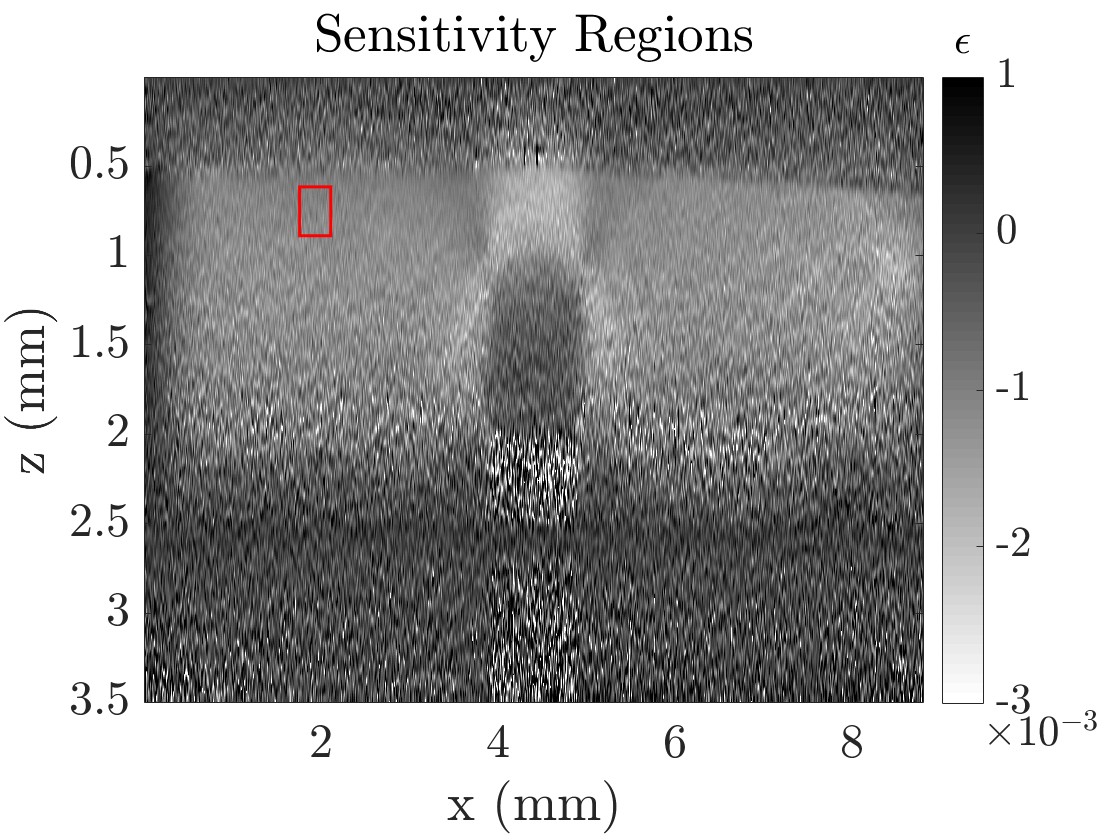
\includegraphics[width=\textwidth]{strainreview_figs/sensitivity_regions.png}
	\end{subfigure}
	\begin{subfigure}{0.49\textwidth}
		\centering
		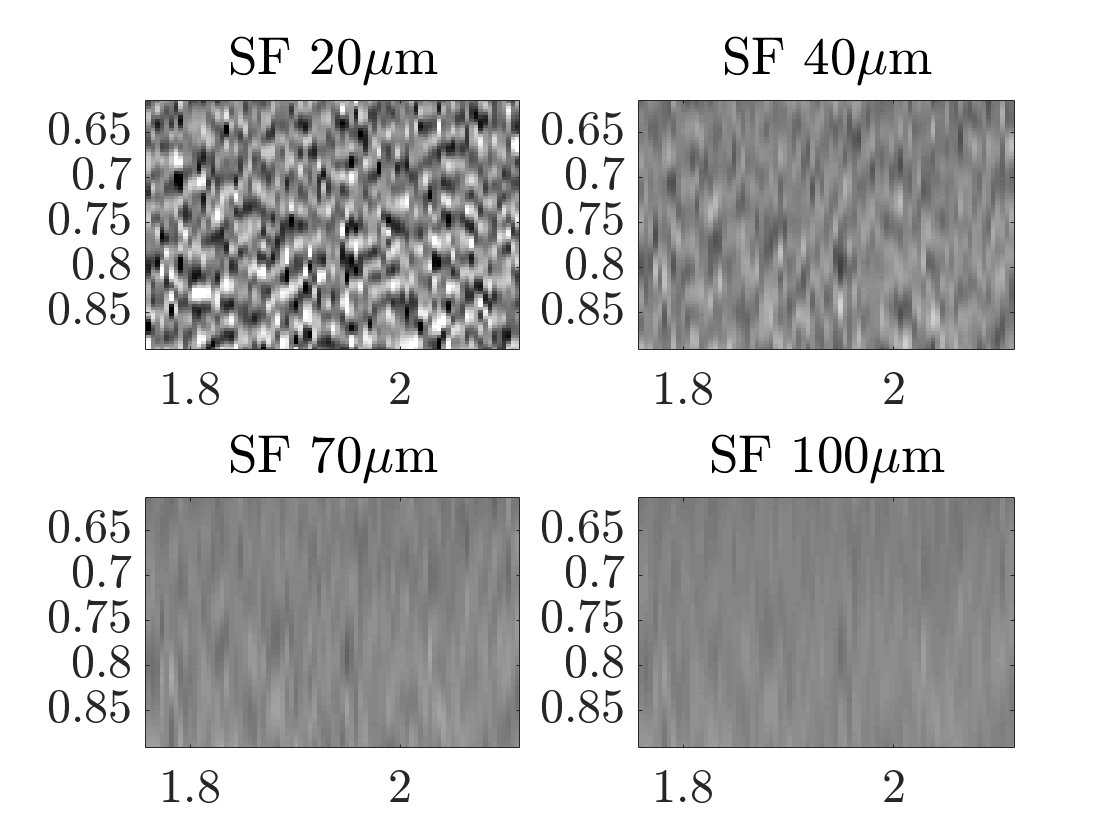
\includegraphics[width=\textwidth]{strainreview_figs/regions_zoomed.png}
	\end{subfigure}
	\caption{A uniform region within a strain elastogram B-scan of a phantom used to measure strain sensitivity, and b) the same region at different fit resolutions. The sensitivity is the standard deviation within the regions, which is higher at strain filter re\ac{fwhm} (SF). The phantom shows high a stiff inclusion (higher strain) surrounded by a softer bulk.}
	\label{sensitivity_region}
\end{figure}

\subsection{Image Resolution}
The image resolution can be thought of as the ability to distinguish between two objects in the resulting strain elastogram. Traditionally, this has been examined in terms of the impulse response of an optical system, more directly as the \ac{fwhm} of this impulse response \cite{reynolds_resolution_1989}. In order to measure the image resolution experimentally, a technique employed in a previous Masters project \cite{hepburn_improving_2017} was employed.

\begin{figure}[t]
	\centering
	\begin{subfigure}{0.49\textwidth}
		\centering
		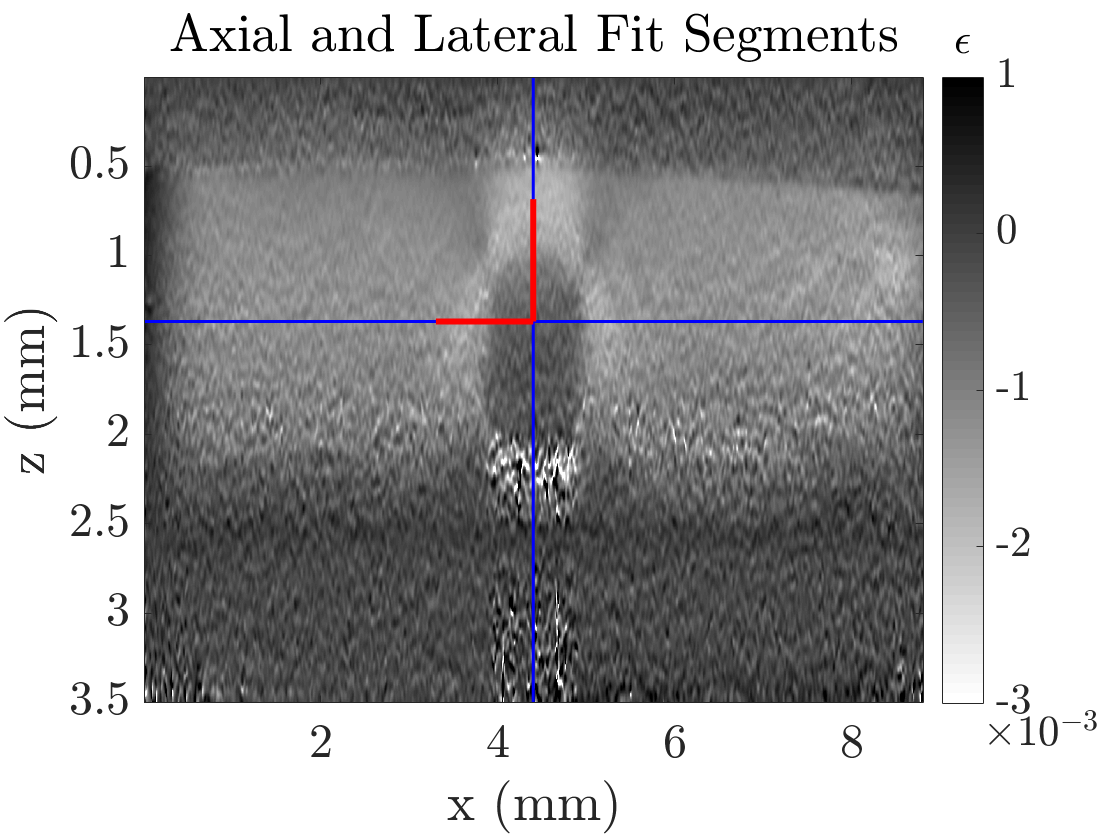
\includegraphics[width=\textwidth]{strainreview_figs/imageres_regions.png}
	\end{subfigure}
	\begin{subfigure}{0.49\textwidth}
		\centering
		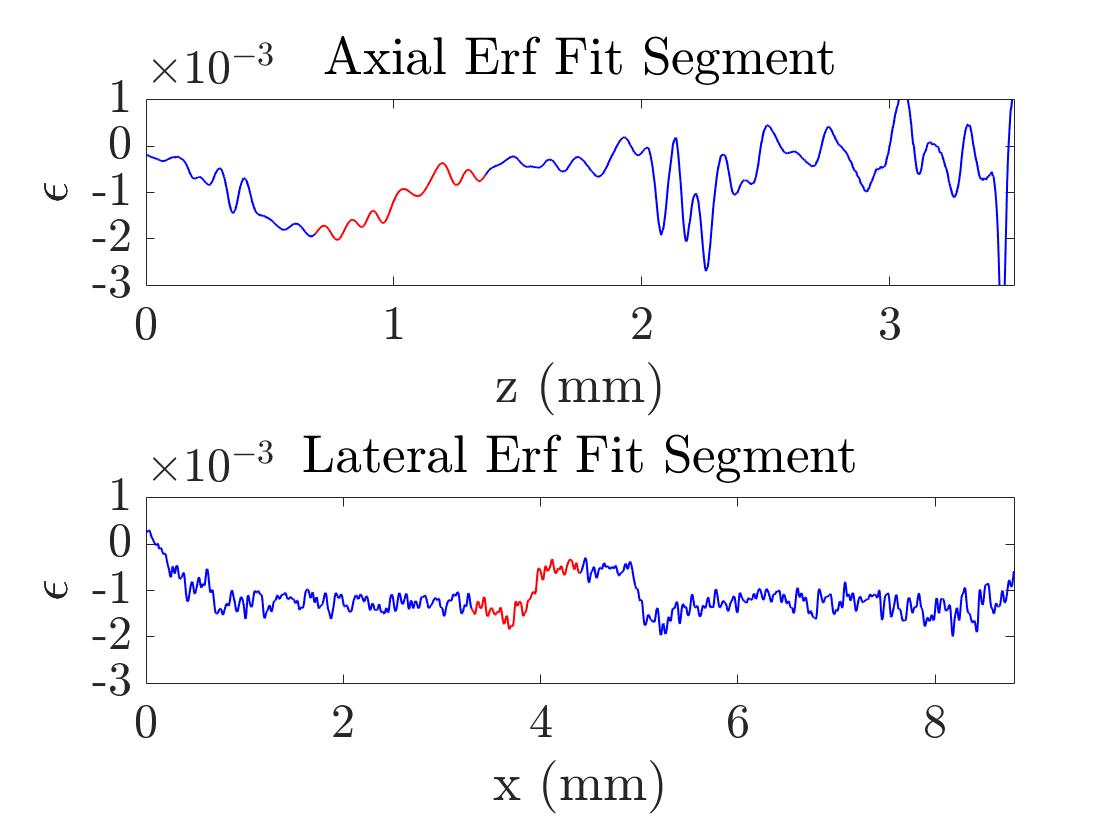
\includegraphics[width=\textwidth]{strainreview_figs/lateral_axial_segments.png}
	\end{subfigure}
	\caption{The segments used to calculate the image resolution for both axial and lateral directions, shown imposed on the strain elastogram on the left, where the blue corresponds to the scan taken, and the red the region the error function is fitted over. The images on the right shows the plots of these scans and segments, with the axial above, and lateral below.}
	\label{axial_lateral_regions}	
\end{figure}

The image resolution is thought of as the `speed' of transition from one uniform strain region to another, as measurable in a phantom sample which has clearly defined regions of different stiffness. This transition can be seen in both the axial and lateral directions, as shown in \autoref{axial_lateral_regions}.

\begin{figure}[t]
	\centering
	\begin{subfigure}{0.49\textwidth}
		\centering
		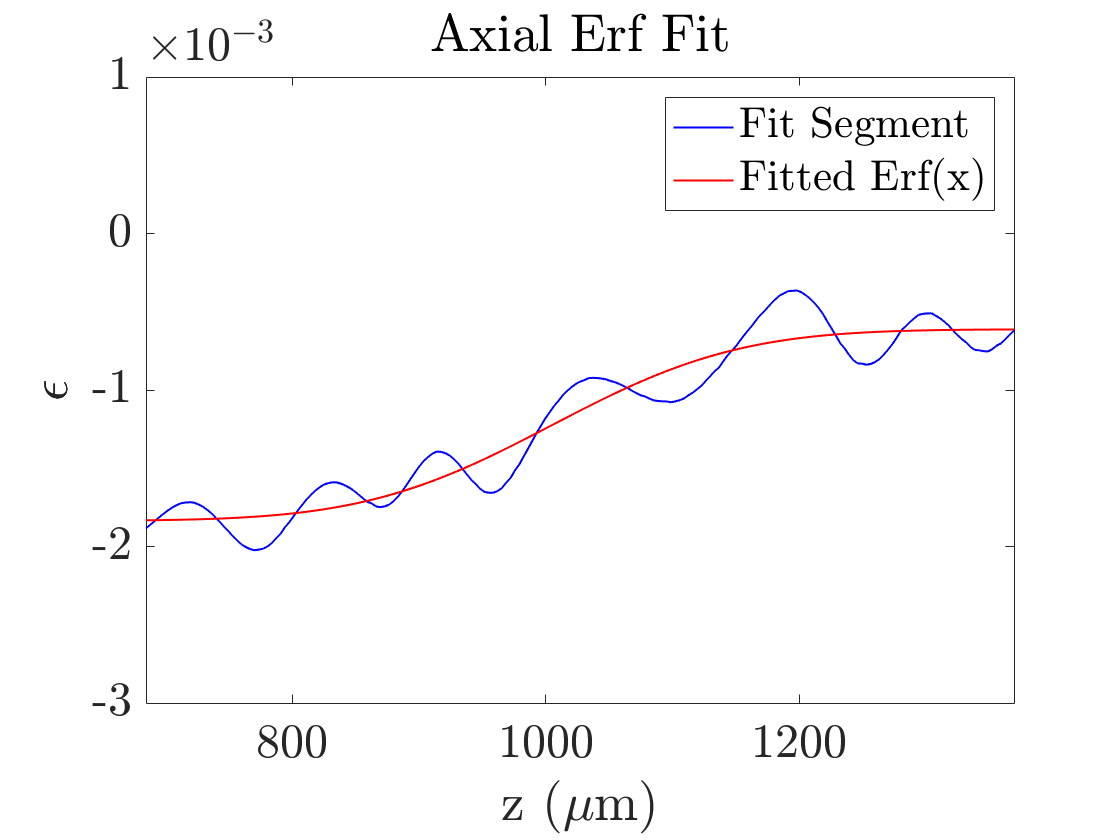
\includegraphics[width=\textwidth]{strainreview_figs/axial_erf_fit.png}
	\end{subfigure}
	\begin{subfigure}{0.49\textwidth}
		\centering
		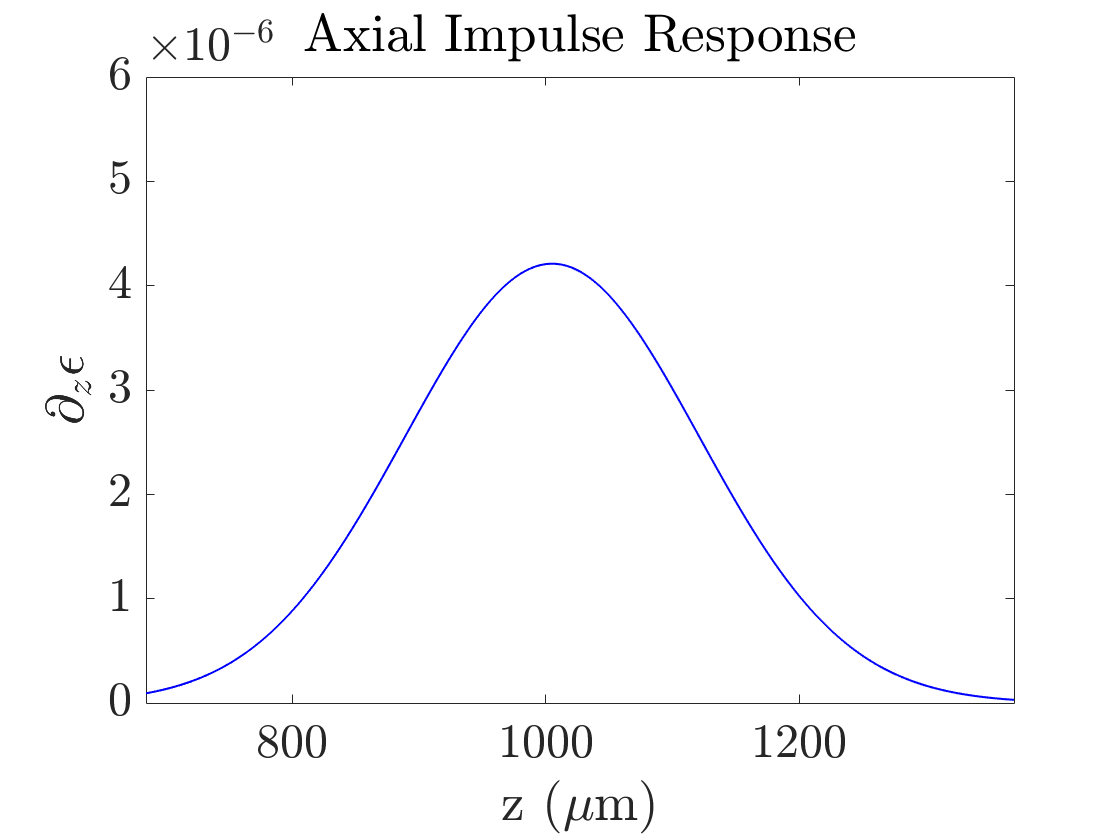
\includegraphics[width=\textwidth]{strainreview_figs/axial_impulse_response.png}
	\end{subfigure}
	\\
	\begin{subfigure}{0.49\textwidth}
		\centering
		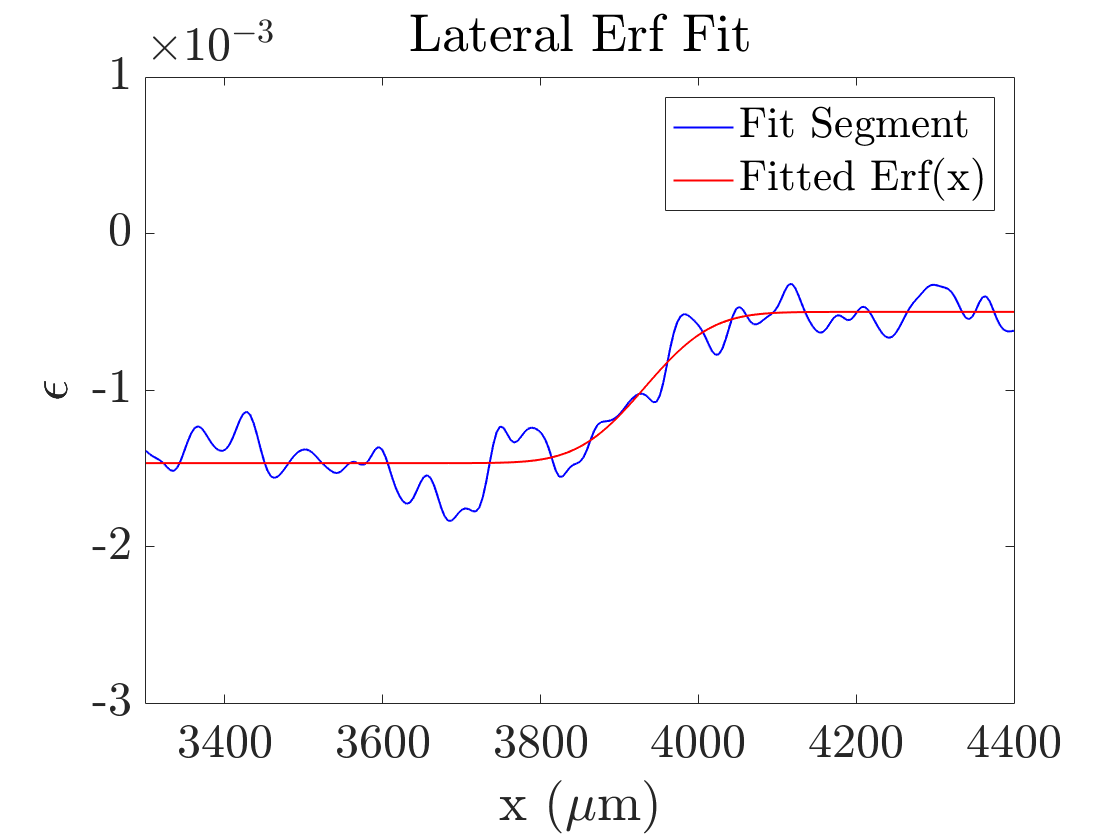
\includegraphics[width=\textwidth]{strainreview_figs/lateral_erf_fit.png}
	\end{subfigure}
	\begin{subfigure}{0.49\textwidth}
		\centering
		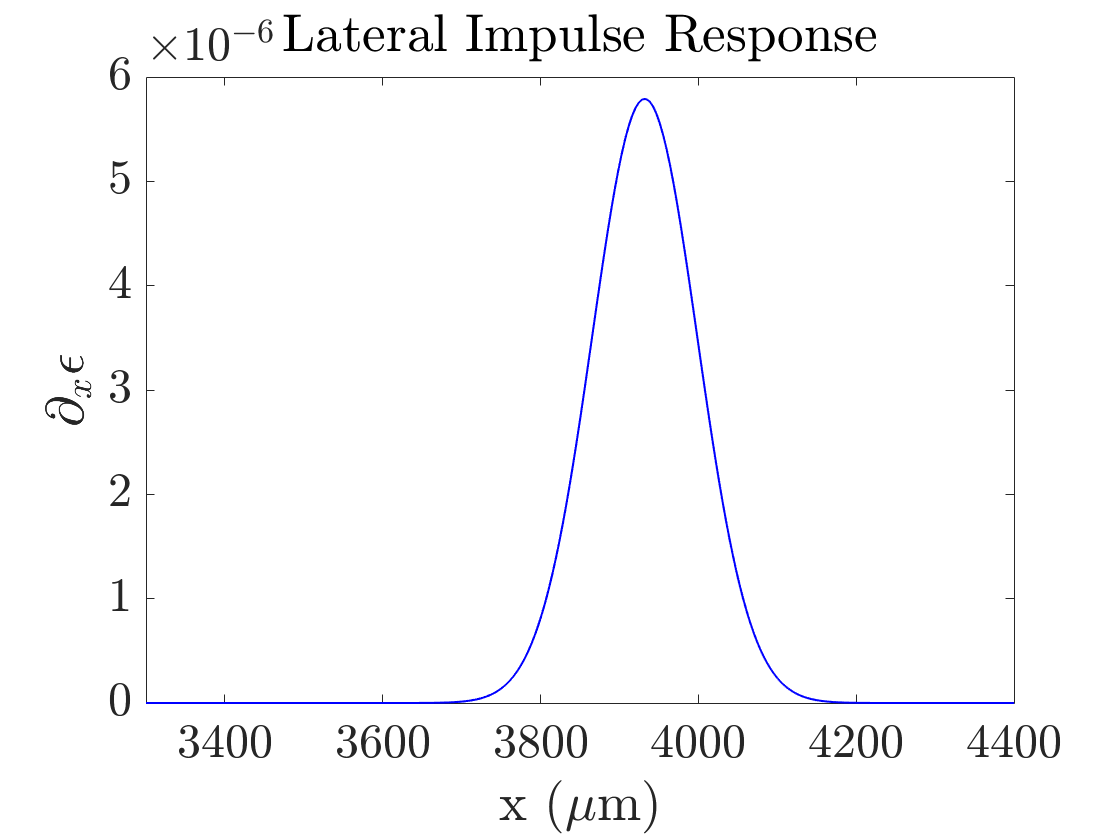
\includegraphics[width=\textwidth]{strainreview_figs/lateral_impulse_response.png}
	\end{subfigure}
	\caption{The left images show the segment over the axial and lateral boundaries respectively with the overlaid error function fit. The right images show the impulse response, which is the derivative of the error function, for the fit, of which the \ac{fwhm} is the image resolution.}
	\label{error_fit_example}	
\end{figure}

The transition across a feature boundary in the strain elastogram can be approximated by an error function, as given in \autoref{erf_normal}, and visualised in \autoref{error_fit_example}. 

\begin{equation}
	\text{erf}(x)=\frac{1}{\sqrt{\pi}} \int_{-x}^{x} \text{e}^{-t^2}
	\label{erf_normal}
\end{equation}

The standard error function above can be translated and scaled (see \autoref{erf_scaled}) to allow fitting to the strain values over the boundary, and also to allow for the introduction of the parameter $a$ that governs the rise time of the error function. When this scaled error function is fitted to the strain data across the boundary, the $a$ parameter is the most significant and is used to calculate an image resolution.

\begin{equation}
	n \: \text{erf}(\:a(x-b)\:) + c = \frac{n}{\sqrt{\pi}} \int_{-(x-b)}^{(x-b)} \text{e}^{-a t^2} + c
	\label{erf_scaled}
\end{equation}

Once this analytical model is derived from the strain data, the derivative of the fitted error function provides the impulse response of the system, and it is the \ac{fwhm} of this derivative that provides the image resolution \cite{hepburn_improving_2017}. For the scaled error function, the derivative is a similarly scaled Gaussian function, given in \autoref{gaussian_derivative}.

\begin{equation}
	G(x) = \frac{2\:a\:n}{\sqrt{\pi}} \text{e}^{-a^2 (x-b)^2}
	\label{gaussian_derivative}
\end{equation}

The \ac{fwhm} of this Gaussian is given in \autoref{image_res_fwhm} and provides the image resolution in the direction specified (axial or lateral, as in \autoref{axial_lateral_regions}).

\begin{equation}
	\text{FWHM}_{IR} = \frac{2 \sqrt{\text{ln}(2)}}{a}
	\label{image_res_fwhm}
\end{equation}

\subsection{Processing Speed}
The processing speed of the strain estimation technique is not a standard metric for assessing the strain elastogram quality, but keeping in mind the motivation for this project it is of utmost importance. To be able to produce strain elastograms in real-time, although Fourier-domain \ac{oct} combined with fast 3D scanning techniques allows for fast data acquisition, the estimation of strain can become a bottleneck in the process that degrades it's application to areas like surgical margin assessment.

The processing speed of the different strain estimation algorithms is assessed by timing the time taken for a single 2D B-scan to process (with 2000 A-scans per B-scan, and ~1000 pixels in depth) as well as for a 3D C-scan (~70 B-scans after spatial averaging). In addition, differences in algorithm complexity are pointed out between the methods, as well as the ease with which they can be parallelised, and the likelihood of a speed up made possible by this parallelisation.
